\documentclass[aspectratio=169]{beamer}

\usepackage[T1]{fontenc}
\usepackage[english]{babel}
\usepackage{dirtytalk}
\usepackage{pgfpages}
\usepackage{listings}
\usepackage{linehighlight}
\usepackage{color}
\usepackage{xparse}
\usepackage{xfp}

\usepackage{blindtext}
\usepackage{lipsum}

\title{Introduction to eBPF}
\author{Martin Ertsås\\ \texttt{martiert@gmail.com}}
\date{\today}

\usetheme{ciscolysaker}
\setbeameroption{show notes on second screen=right}

\definecolor{codehighlight}{rgb}{0.8, 0.95, 0.8}
\definecolor{codebackground}{rgb}{0.9, 0.9, 0.9}


\usepackage{graphicx}

\lstdefinelanguage{diff}{
 morecomment=[f][\color{Green}]{+},
 morecomment=[f][\color{Red}]{-},
}

\lstdefinelanguage{asm}{
  morekeywords={load, jmp, jeq, jge, jgt, ret},
}
\lstdefinestyle{cpp}{
  language=C++,
  morekeywords={
    __u32,
    __u64,
    __s32,
    __s64,
    uint8_t,
    uint16_t,
    uint32_t,
    uint64_t,
    int8_t,
    int16_t,
    int32_t,
    int64_t,
  },
}

\lstset{
 frame=single,
 language=diff,
 morekeywords={uint8_t, ssize_t},
 keywordstyle=\color{Blue},
 showspaces=false,
 showstringspaces=false,
 backgroundcolor=\color{codebackground},
 literate={å}{{\aa}}1
}
\newenvironment{SplitView}[2]
  {
    \begin{columns}
      \begin{column}{0.35\textwidth}
        \centering
        \includegraphics[height=0.8\textheight, width=\textwidth, keepaspectratio]{#1}
      \end{column}
      \begin{column}{0.65\textwidth}
        {\Large\color{Blue}{#2}}
        \vskip 1em
  }
  {
      \end{column}
    \end{columns}
  }
\newenvironment{RotateSplitView}[2]
  {
    \begin{columns}
      \begin{column}{0.35\textwidth}
        \centering
        \includegraphics[angle=90, height=0.8\textheight, width=\textwidth, keepaspectratio]{#1}
      \end{column}
      \begin{column}{0.65\textwidth}
        {\Large\color{Blue}{#2}}
        \vskip 1em
  }
  {
      \end{column}
    \end{columns}
  }

\newcommand{\demo}[1]{\begin{frame}{DEMO!}\note{#1}\end{frame}}

\begin{document}

\begin{frame}
  \titlepage

  \note{
    \begin{itemize}
      \item Ask questions whenever
      \item Feel free to interrupt
      \item If I forget breaks, shout out
    \end{itemize}
  }
\end{frame}

\begin{frame}
  \begin{SplitView}{images/mertsas.jpg}{\$ Whoami}
    \centering
    \lstinputlisting[basicstyle=\small]{examples/whoami.txt}
  \end{SplitView}

  \note{
    \begin{itemize}
      \item Works for Cisco Norway
      \item Been working a couple years now with integrating chromium in our embedded devices
      \item Mainly interested in systems programming, security, and training
      \item Likes board games, RPG games, and cycling
    \end{itemize}
  }
\end{frame}

\begin{frame}
  \begin{SplitView}{images/important.jpg}{I have no idea what I'm doing}
    \begin{itemize}
      \item<2-> I wanted to experiment with eBPF
      \item<2-> So I submitted this talk
      \item<2-> This might have been a mistake
      \item<2-> Definitely do not use any code from this presentation
      \item<2-> It will blow up in your face
    \end{itemize}
  \end{SplitView}

  \note{
  }
\end{frame}

\begin{frame}
  \begin{SplitView}{images/question.jpg}{What is eBPF?}
    \begin{itemize}
      \item A way to program the kernel without building a new kernel or writing kernel modules
      \item A programing language, evaluated by the kernel
      \item Event driven programs, running when the kernel passes a pre-defined hook
      \item Can be controlled from userspace
    \end{itemize}
  \end{SplitView}

  \note{
    Write kernel features without:

    \begin{itemize}
      \item Modifying the kernel
      \item Submit the patch upstream
      \item Wait for kernel release
      \item Wait for distro to pick up the new kernel
    \end{itemize}
  }
\end{frame}

\begin{frame}
  \begin{SplitView}{images/break wall.png}{Can I harm the kernel?}
    \begin{itemize}
      \item Process loading the eBPF program needs correct capabilities
      \item Runs through a verifyer on every program load
        \begin{itemize}
          \item The program does not crash or harm the system
          \item No use of uninitialized memory
          \item Program is withing size limit
          \item Program has finite complexity
        \end{itemize}
      \item Memory for ebpf program itself is read-only
      \item Runs in an protected execution context
    \end{itemize}
  \end{SplitView}

  \note{
    \begin{itemize}
      \item Mainly need CAP\_BPF, can also allow unprivileged for certain hooks
      \item Finite complexity means we for instance can't have infinite loops and we always run to completion
      \item Not possible to modify ebpf program
      \item No access to arbitrary kernel memory
      \item Need to use helper functions to get memory outside of execution context
    \end{itemize}
  }
\end{frame}

\begin{frame}
  \begin{SplitView}{images/question.jpg}{Why would you like to use this?}
    \begin{itemize}
      \item Monitoring and tracing of processes
      \item Network monitoring
      \item Making network decisions
      \item To be one of the cool kids
    \end{itemize}
  \end{SplitView}

  \note{
    Our use case was to put a specific process into a cgroup on creation, to limit its memory usage
  }
\end{frame}

\begin{frame}{ebpf architecture}
  \centering
  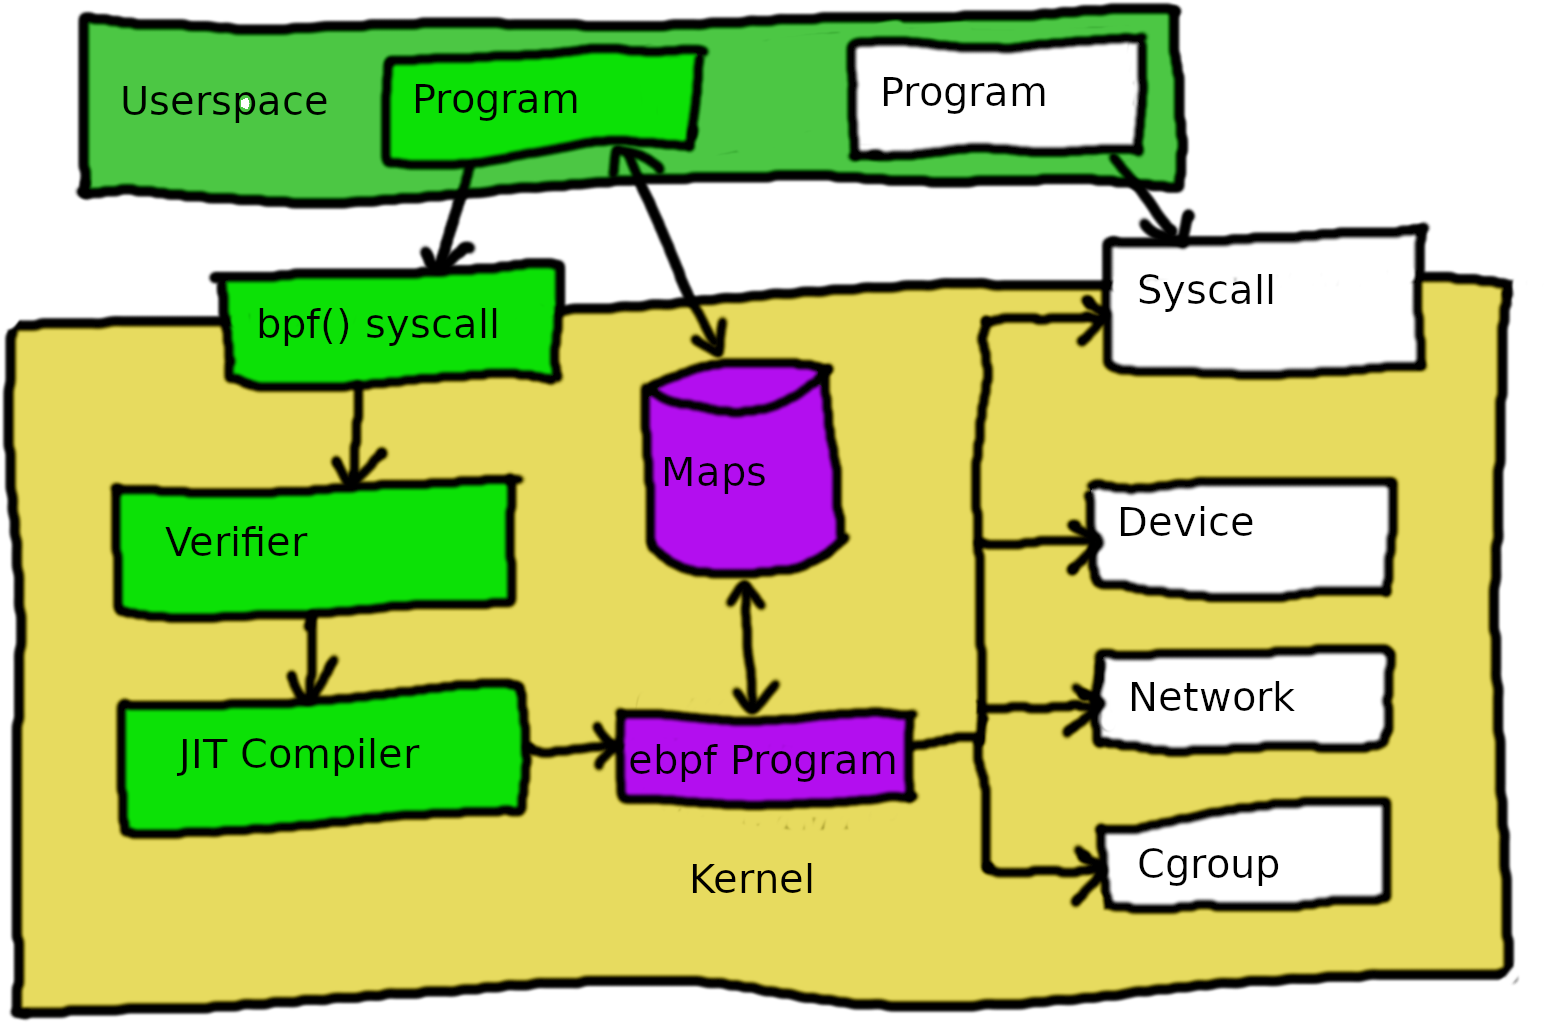
\includegraphics[width=0.7\textwidth, keepaspectratio]{images/ebpf.png}
\end{frame}

\begin{frame}
  \begin{RotateSplitView}{images/chaos.png}{Abstractions and tools}
    \begin{itemize}
      \item libbpf
      \item bpftool
      \item bcc
      \item clang
      \item netlink
    \end{itemize}
  \end{RotateSplitView}

  \note{
  }
\end{frame}

\begin{frame}{Simple ebpf program}
  \lstinputlisting[basicstyle=\small, language=C]{examples/simple.ebpf.c}

  \note{
    \begin{itemize}
      \item $SEC$ defines an ELF section to use
      \item A GPL compatible license is required
      \item $BPF_CORE_READ$ reads entries from a struct
      \item bpf\_probe\_read\_kernel\_str copies from an unsafe kernel address
    \end{itemize}
  }
\end{frame}

\begin{frame}{Simple loading program}
  \lstinputlisting[language=C]{examples/simple.host.c}

  \note{
    The simple\_\_ functions are auto generated from the ebp program using bpftool
  }
\end{frame}

\demo{
  \begin{itemize}
    \item bpftool prog to show that it is loaded
    \item cat /sys/kernel/debug/tracing/trace\_pipe
  \end{itemize}
}

\begin{frame}
  \begin{SplitView}{images/phone.png}{Communicate to userspace}
    \begin{itemize}
      \item .bss section
      \item ebpf maps
    \end{itemize}
  \end{SplitView}
\end{frame}

\begin{frame}
  \begin{SplitView}{images/chain.png}{}
    \lstinputlisting[caption=ebpf]{examples/bss.diff}
    \lstinputlisting[caption=userspace]{examples/bss.host.diff}
  \end{SplitView}

  \note{
    \begin{itemize}
      \item Adding an integer to the .bss section
      \item Using that from the ebpf program
      \item Exposed in the skeleton on the host side
      \item Pretty much one-way
      \item Very limited
    \end{itemize}
  }
\end{frame}

\begin{frame}
  \begin{SplitView}{images/map.png}{ebpf maps}
    \begin{itemize}
      \item Multiple map types
    \end{itemize}
  \end{SplitView}
\end{frame}

\begin{frame}
  \begin{SplitView}{images/map.png}{Creating a map}
    \lstinputlisting{examples/ringbuffer.define.diff}
  \end{SplitView}
\end{frame}

\begin{frame}
  \begin{SplitView}{images/map.png}{Creating a map}
    \lstinputlisting{examples/ringbuffer.bpf.diff}
  \end{SplitView}
\end{frame}

\begin{frame}
  \begin{SplitView}{images/map.png}{Reading a ringbuffer from ebpf}
    \lstinputlisting{examples/ringbuffer.userspace.diff}
  \end{SplitView}
\end{frame}

\begin{frame}
  \begin{SplitView}{images/mertsas.jpg}{Consuming data}
    \lstinputlisting[language=C]{examples/ringbuffer.callback.cpp}
  \end{SplitView}
\end{frame}

\demo{}

\begin{frame}
  \begin{SplitView}{images/phone.png}{Communicating from userspace}
    \begin{itemize}
      \item Very similar to communicating to userspace
      \item Can send over more complex types
      \item Can easily keep several entries
    \end{itemize}
  \end{SplitView}
\end{frame}

\begin{frame}
  \begin{SplitView}{images/phone.png}{Path of commands map}
    \lstinputlisting{examples/command\_name.ebpf.diff}
  \end{SplitView}
\end{frame}

\begin{frame}
  \begin{SplitView}{images/phone.png}{Using the commands map}
    \lstinputlisting{examples/command\_name.ebpf.check.diff}
  \end{SplitView}
\end{frame}

\begin{frame}
  \begin{SplitView}{images/phone.png}{Populating from userspace}
    \lstinputlisting{examples/command\_name.userspace.diff}
  \end{SplitView}
\end{frame}

\demo{}

\begin{frame}
  \begin{SplitView}{images/mertsas.jpg}{Putting the process into a cgroup}
    \begin{itemize}
      \item Can easily be done in userspace at this point
      \item Need to clean up when it exits
      \item Add a program for system exit
      \item Keep a map to communicate between the two programs
    \end{itemize}
  \end{SplitView}

  \note{
    Going to be lazy and not show it

    Show an example of a run, and show the folder that is created
  }
\end{frame}

\begin{frame}
  \begin{SplitView}{images/mertsas.jpg}{Internal monitoring map}
    \lstinputlisting{examples/monitor\_map.diff}
  \end{SplitView}
\end{frame}

\begin{frame}
  \begin{SplitView}{images/mertsas.jpg}{Populate monitoring}
    \lstinputlisting{examples/monitor\_populate.diff}
  \end{SplitView}

  \note{
    bpf\_map\_update\_elem NOEXIST only updates if the key doesn't exist.
  }
\end{frame}

\begin{frame}
  \begin{SplitView}{images/mertsas.jpg}{Handling exit syscall}
    \lstinputlisting[language=C]{examples/sched\_process\_exit.c}
  \end{SplitView}

  \note{
    First thing we do is try to remove the pid from the list of monitored pids

    If we fail to remove it, it doesn't exist and we exit

    Send an exit event for the pid to userspace

    Userspace can then use the new type enum to remove the cgroup folder
  }
\end{frame}

\begin{frame}
  \begin{SplitView}{images/mertsas.jpg}{Currently only used tracepoints}
    \begin{itemize}
      \item Can connect programs to the cgroup itself
      \item Or to a network interface+++
    \end{itemize}
  \end{SplitView}
\end{frame}

\begin{frame}
  \begin{SplitView}{images/mertsas.jpg}{cgroup network programs}
    \lstinputlisting[basicstyle=\small]{examples/cgroup\_network.diff}
  \end{SplitView}
\end{frame}

\begin{frame}
  \begin{SplitView}{images/mertsas.jpg}{Connecting ingress and egress}
    \lstinputlisting[language=C]{examples/attach\_cgroup.c}
  \end{SplitView}
\end{frame}

\begin{frame}
  \begin{SplitView}{images/Wictor.jpg}{Thank you}
  \end{SplitView}
\end{frame}

\end{document}
